\documentclass[lettersize,journal]{IEEEtran}
\usepackage{amsmath,amsfonts}
\usepackage{algorithmic}
\usepackage{algorithm}
\usepackage{array}
\usepackage[caption=false,font=normalsize,labelfont=sf,textfont=sf]{subfig}
\usepackage{textcomp}
\usepackage{stfloats}
\usepackage{url}
\usepackage{verbatim}
\usepackage{graphicx}
\usepackage{cite}
\usepackage{hyperref}
\usepackage{tikz}
\usetikzlibrary{shapes.geometric, arrows.meta, positioning, calc, patterns}
\usepackage{color}
\usepackage{listings}
% 定义MATLAB代码块颜色
\definecolor{codegreen}{rgb}{0,0.6,0}
\definecolor{codegray}{rgb}{0.5,0.5,0.5}
\definecolor{codepurple}{rgb}{0.58,0,0.82}
\definecolor{backcolour}{rgb}{0.95,0.95,0.92}
% 定义MATLAB代码样式
\lstdefinestyle{mystyle}{
    backgroundcolor=\color{backcolour},   
    commentstyle=\color{codegreen},
    keywordstyle=\color{magenta},
    numberstyle=\tiny\color{codegray},
    stringstyle=\color{codepurple},
    basicstyle=\ttfamily\footnotesize,
    breakatwhitespace=false,         
    breaklines=true,                 
    captionpos=b,                    
    keepspaces=true,                 
    numbers=left,                    
    numbersep=5pt,                  
    showspaces=false,                
    showstringspaces=false,
    showtabs=false,                  
    tabsize=2
}
% 设置代码样式
\lstset{style=mystyle}
\hyphenation{op-tical net-works semi-conduc-tor IEEE-Xplore}
% updated with editorial comments 8/9/2021

\begin{document}

\title{Capacity of MIMO Channels with Known CSIT}

\author{Name: Shuao Chen, Student ID: 023034910028, Email: shuao.chen@sjtu.edu.cn
        % <-this % stops a space
}

% The paper headers
\markboth{Academic Writing, Norms, and Ethics}%
{Shell \MakeLowercase{\textit{et al.}}: A Sample Article Using IEEEtran.cls for IEEE Journals}

% Remember, if you use this you must call \IEEEpubidadjcol in the second
% column for its text to clear the IEEEpubid mark.

\maketitle

\begin{abstract}
This study addresses the channel capacity enhancement in MIMO systems, leveraging the concept of CSIT. Utilizing the waterfilling algorithm, the research analytically investigates the capacity optimization for various MIMO channel matrices under different SNR conditions. Through a detailed SVD of the channel matrices, the work presents an algorithmic approach to distribute transmission power efficiently across the channel eigenmodes, thereby maximizing the capacity. The simulation results demonstrate a logarithmic increase in capacity with SNR and reveal the significance of channel diversity and CSIT in capacity enhancement. The findings confirm the effectiveness of the waterfilling algorithm, showing substantial gains in the capacity of MIMO channels, with an in-depth discussion on the influence of eigenmode structures and SNR levels. These results contribute to the advancement of adaptive transmission strategies, offering a comprehensive understanding for future wireless communication systems optimization.
\end{abstract}

\begin{IEEEkeywords}
MIMO, channel capacity, waterfilling algorithm.
\end{IEEEkeywords}

\section{Introduction}
\IEEEPARstart{M}{ultiple} Input Multiple Output (MIMO) systems represent a significant advancement in wireless communication technology. Characterized by their use of multiple antennas at both the transmitter and receiver ends, MIMO systems exploit spatial diversity to enhance communication performance\cite{lu2014overview}. This spatial diversity enables MIMO systems to achieve higher data throughput and increased link reliability compared to traditional single-antenna systems. The underlying principle of MIMO technology is to utilize multiple transmission and reception paths to transmit more data simultaneously, effectively increasing the capacity of the communication channel.

Channel State Information (CSI) plays a pivotal role in optimizing the performance of wireless communication systems, particularly in the context of MIMO technologies\cite{shen2016compressed}. CSI comprises the knowledge of channel properties, including how a signal propagates from the transmitter to the receiver and the effects of various channel impairments such as fading and path loss. The accurate estimation and utilization of CSI are crucial for effectively decoding the received signal and adapting transmission strategies to current channel conditions. CSI can be categorized into two types: CSI at the Receiver (CSIR), which is used to optimize signal decoding, and CSI at the Transmitter (CSIT), which is crucial for adaptive transmission strategies.

The incorporation of CSIT in MIMO systems enables a more sophisticated and efficient use of the communication channel. With the knowledge of the channel state at the transmitter side, adaptive transmission techniques, such as precoding and power control, can be employed. These techniques allow for the adjustment of the transmitted signals based on the channel conditions, thereby maximizing the efficiency of power and bandwidth utilization. CSIT enables the transmitter to adaptively modify the signal in a way that mitigates detrimental channel effects, leading to improved signal quality at the receiver and an overall increase in system capacity.

Channel capacity, a fundamental concept in information theory, quantifies the maximum rate at which information can be reliably transmitted over a communication channel. In MIMO systems, channel capacity is influenced by several factors, including the number of transmit and receive antennas, channel conditions, and the availability of CSIT\cite{goldsmith2003capacity}. The Shannon-Hartley theorem lays the foundation for understanding channel capacity, indicating that it increases with the signal-to-noise ratio (SNR) and bandwidth\cite{rioul2014shannon}. The calculation of channel capacity in MIMO systems, especially with known CSIT, involves sophisticated mathematical models that account for the spatial multiplexing of signals and the allocation of power across multiple transmission paths. The use of techniques such as the water-filling algorithm in the context of CSIT allows for the optimal distribution of power among different channel eigenmodes, further enhancing the channel capacity\cite{lu2013water}.

\section{MIMO System Model}
In the context of a MIMO system with \( N_t \) transmitting antennas and \( N_r \) receiving antennas, as depicted in Fig. \ref{fig:MIMOSystem}, the system dynamics can be elaborated as follows:

Consider the transmission matrix \( \mathbf{X} \) to be an \( N_t \times 1 \) column matrix, where \( X_i \) represents the ith component transmitted from the ith antenna. In scenarios where the channel is characterized as a Gaussian channel with its elements being independent and identically distributed (\textit{i.i.d.}) Gaussian variables, and the channel state is unknown at the transmitter, a uniform power distribution strategy is adopted. Specifically, each transmitting antenna is allocated an equal power fraction of \( \frac{P_t}{N_t} \), where \( P_t\) denotes the total transmitter power, independent of the number of antennas. The covariance matrix of the transmitted matrix is given by:
\begin{equation}
\mathbf{R}_{xx} = \frac{P_t}{N_t} \mathbf{I}_{N_t}
\end{equation}
where \( \mathbf{I}_{N_t} \) is an \( N_t \times N_t \) identity matrix. Considering the narrow bandwidth of the transmitted signal, the channel is assumed to be flat. The channel matrix \( \mathbf{H} \) is thus defined as an \( N_t \times N_r \) complex matrix, with the matrix component \( h_{i,j} \) representing the fading coefficient from the jth transmit antenna to the ith receiver. In situations where the channel matrix is only known at the receiver end, it can be estimated through a training sequence. Should there be a need for the transmitter to acquire this channel information, it can be communicated back to the transmitter via a feedback channel\cite{liao2019csi}.

\begin{figure}[!t]
\centering
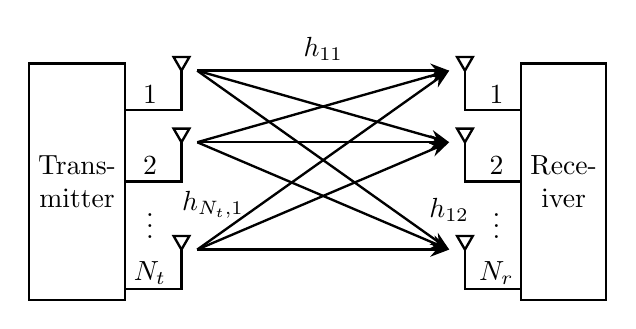
\begin{tikzpicture}[>=Stealth, line width=0.3mm]

% Transmitter and receiver blocks
\node (tx) [draw, rectangle, minimum height=3cm, minimum width=1cm, align=center] {Trans-\\mitter};
\node (rx) [draw, rectangle, minimum height=3cm, minimum width=1cm, right=5cm of tx, align=center] {Rece-\\iver};

\coordinate (tx1) at ($(tx.north east)!0.4!(tx.east)$);
\coordinate (tx2) at ($(tx.north east)!1!(tx.east)$);
\coordinate (tx3) at ($(tx.east)!0.9!(tx.south east)$);
\draw (tx1) -- ++(0:0.7) -- ++(90:0.5) coordinate (txan1);
\draw (tx2) -- ++(0:0.7) -- ++(90:0.5) coordinate (txan2);
\draw (tx3) -- ++(0:0.7) -- ++(90:0.5) coordinate (txan3);
\draw (txan1) -- ++(60:0.2) -- ++(0:-0.2) -- cycle;
\draw (txan2) -- ++(60:0.2) -- ++(0:-0.2) -- cycle;
\draw (txan3) -- ++(60:0.2) -- ++(0:-0.2) -- cycle;

\coordinate (rx1) at ($(rx.north west)!0.4!(rx.west)$);
\coordinate (rx2) at ($(rx.north west)!1!(rx.west)$);
\coordinate (rx3) at ($(rx.west)!0.9!(rx.south west)$);
\draw (rx1) -- ++(0:-0.7) -- ++(90:0.5) coordinate (rxan1);
\draw (rx2) -- ++(0:-0.7) -- ++(90:0.5) coordinate (rxan2);
\draw (rx3) -- ++(0:-0.7) -- ++(90:0.5) coordinate (rxan3);
\draw (rxan1) -- ++(60:0.2) -- ++(0:-0.2) -- cycle;
\draw (rxan2) -- ++(60:0.2) -- ++(0:-0.2) -- cycle;
\draw (rxan3) -- ++(60:0.2) -- ++(0:-0.2) -- cycle;

\draw[->] ([xshift=0.2cm] txan1.east) -- ([xshift=-0.2cm] rxan1.west) node[midway, above] {$h_{11}$};
\draw[->] ([xshift=0.2cm] txan1.east) -- ([xshift=-0.2cm] rxan2.west);
\draw[->] ([xshift=0.2cm] txan1.east) -- ([xshift=-0.2cm] rxan3.west) node[xshift=0cm,yshift=0.5cm] {$h_{12}$};
\draw[->] ([xshift=0.2cm] txan2.east) -- ([xshift=-0.2cm] rxan1.west);
\draw[->] ([xshift=0.2cm] txan2.east) -- ([xshift=-0.2cm] rxan2.west);
\draw[->] ([xshift=0.2cm] txan2.east) -- ([xshift=-0.2cm] rxan3.west);
\draw[->] ([xshift=0.2cm] txan3.east) -- ([xshift=-0.2cm] rxan1.west) node[xshift=-3.0cm,yshift=-1.7cm] {$h_{N_t,1}$};
\draw[->] ([xshift=0.2cm] txan3.east) -- ([xshift=-0.2cm] rxan2.west);
\draw[->] ([xshift=0.2cm] txan3.east) -- ([xshift=-0.2cm] rxan3.west);

\node at ([xshift=0.4cm, yshift=0.4cm]rxan3) {\vdots};
\node at ([xshift=-0.4cm, yshift=0.4cm]txan3) {\vdots};
\node at ([xshift=-0.4cm, yshift=-0.3cm]txan1) {1};
\node at ([xshift=-0.4cm, yshift=-0.3cm]txan2) {2};
\node at ([xshift=-0.4cm, yshift=-0.3cm]txan3) {$N_t$};
\node at ([xshift=0.4cm, yshift=-0.3cm]rxan1) {1};
\node at ([xshift=0.4cm, yshift=-0.3cm]rxan2) {2};
\node at ([xshift=0.4cm, yshift=-0.3cm]rxan3) {$N_r$};
\end{tikzpicture}
\caption{Simplified MIMO system.}
\label{fig:MIMOSystem}
\end{figure}

In the discussed MIMO system, the noise at the receiver is represented by another column vector of size \( N_r \times 1 \), denoted as \( \mathbf{n} \). The components of \( \mathbf{n} \) are assumed to have zero mean and circular symmetry. The analysis omits factors such as antenna gain, signal attenuation, and other complexities for a deterministic channel. The received signal at the ith receiver, considering \( N_t \) transmitting antennas, is thus modeled as:
\begin{equation}
r_i = \sum_{j=1}^{N_t} h_{ij} x_j, \quad i = 1, 2, 3, \ldots
\end{equation}

The covariance matrix of the receiver noise is given by:
\begin{equation}
\mathbf{R}_{nn} = \mathbb{E}\left[\mathbf{n} \mathbf{n}^H\right]
\end{equation}

In the case of uncorrelated noise components, the receiver noise covariance matrix simplifies to:
\begin{equation}
\mathbf{R}_{nn} = \sigma_n \mathbf{I}_{N_r}
\end{equation}
where \( \sigma_n\) represents the noise power in each of the \( N_r \) receive branches, and \( \mathbf{I}_{N_r} \) is the \( N_r \times N_r \) identity matrix. Under the assumption that the total received power per antenna equals the total transmitted power, the SNR can be expressed as:
\begin{equation}
\gamma = \frac{E_t}{N_t}
\end{equation}

Thus, the receiver vector can be expressed as:
\begin{equation} \label{eq:sysequ}
\mathbf{y} = \mathbf{Hx} + \mathbf{n}
\end{equation}

The \( N_r \times N_t \) channel matrix, with elements \( h_{ji} \), representing the channel response, is denoted as:

\begin{equation}
\mathbf{H} = 
\begin{bmatrix}
h_{1,1} & h_{1,2} & \ldots & h_{1,N_t} \\
h_{2,1} & h_{2,2} & \ldots & h_{2,N_t} \\
\vdots  & \vdots  & \ddots & \vdots  \\
h_{N_r,1} & h_{N_r,2} & \ldots & h_{N_r,N_t}
\end{bmatrix}
\end{equation}
where \( h_{j,i} \) is the complex channel coefficient between the \textit{i}-th antenna at the transmitter and the \textit{j}-th antenna at the receiver side, characterized as having zero mean, circular symmetry, and complex Gaussian distribution.

\section{Channel Is Known to the Transmitter}
In certain scenarios, the transmitter can acquire CSI, significantly enhancing the system's performance. When CSI is available at the transmitter, the channel capacity can be increased by implementing the water-filling principle. This technique involves allocating varying levels of power to the transmitting antennas based on the quality of their respective channels. Essentially, channels with better conditions receive more power, while those with poorer conditions receive less, or possibly no power at all.

With known channel parameters at the transmitter, the waterfilling algorithm serves as a tool to optimize channel capacity. It achieves this by preferentially allocating more power to channels in good condition, and less or none to those in poor condition. This strategy is particularly effective in narrowband channels.

Given the channel matrix \( \mathbf{H} \), its Singular Value Decomposition (SVD) can be expressed as \( \mathbf{H} = \mathbf{USV}^H \)\cite{lebrun2005mimo}, where:
\begin{itemize}
    \item \( \mathbf{U} \) and \( \mathbf{V} \) are unitary matrices containing the eigenvectors of the receiver and transmitter, respectively.
    \item \( \mathbf{S} \) is a diagonal matrix containing the singular values \( \lambda_i \) of \( \mathbf{H} \).
\end{itemize}

As illustrated in Fig. \ref{fig:waterfilling}, the waterfilling algorithm allocates power across different channels based on the noise level of each channel. The transmitted vector \( \mathbf{x} \) is pre-multiplied by \( \mathbf{V} \) to counteract the effect of \( \mathbf{V}^H \) in \( \mathbf{H} \), and the received vector \( \mathbf{y} \) is post-multiplied by \( \mathbf{U}^H \) to negate the influence of \( \mathbf{U} \) in \( \mathbf{H} \). Thus, the transformed system can be represented as:
\begin{equation}
\mathbf{\tilde{x}} = \mathbf{Vx}, \quad \mathbf{\tilde{y}} = \mathbf{U}^H\mathbf{y}, \quad \mathbf{\tilde{n}} = \mathbf{U}^H\mathbf{n}
\end{equation}

Substituting these values into the system equation \eqref{eq:sysequ} yields:
\begin{equation}
\mathbf{\tilde{y}} = \mathbf{S\tilde{x}} + \mathbf{\tilde{n}}
\end{equation}

This formulation effectively represents a set of parallel Single-Input Single-Output (SISO) channels, where the power gains are the non-zero diagonal elements of the matrix \( \mathbf{S} \). Consequently, the capacity of the MIMO channel, denoted as \( C_\text{MIMO} \), is the aggregate of the capacities of these individual parallel SISO channels. The power transmitted over each eigenvalue \( \lambda_i \) is allocated such that:
\begin{equation}
C_\text{MIMO} = \sum_{i=1}^{n} \text{capacity of each SISO channel}
\end{equation}

Maximizing the channel capacity involves the transmitter accessing individual subchannels, represented by the eigenvalues, and allocating variable power levels to them. Therefore, the problem of mutual information maximization can be formulated as:
\begin{equation} \label{eq:capacity}
\begin{aligned}
\max_{P_i} \quad & \sum_{i=1}^{\text{rank}(\mathbf{H})} \log_2 \left(1 + \frac{\lambda_i^2 P_i}{\sigma_n^2}\right) \\
\text{s.t.} \quad & \sum_{i=1}^{\text{rank}(\mathbf{H})} P_i \leq P_t
\end{aligned}
\end{equation}
Utilizing the Lagrangian method, the optimal energy allocation to each eigenmode is determined. The optimal power \( P_{\text{opt},i} \) for each eigenmode is given by:
\begin{equation} \label{eq:popt}
P_{\text{opt},i} = \left( \mu - \frac{\sigma_n^2}{\lambda_i^2} \right)^+
\end{equation}
and
\begin{equation} \label{eq:psum}
\sum_{i=1}^{\text{rank}(\mathbf{H})} P_{\text{opt},i} = P_{t}
\end{equation}
Here, \( \mu \) is a constant representing the water level, and the operation \( (x)^+ \) is defined as:
\begin{equation}
(x)^+ = 
\begin{cases} 
x & \text{if } x \geq 0 \\
0 & \text{if } x < 0
\end{cases}
\end{equation}

\begin{figure}[!t]
\centering
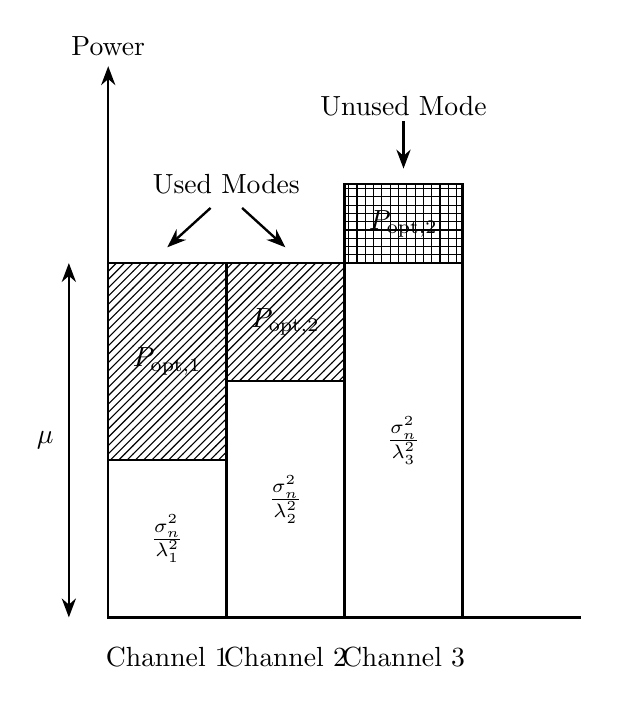
\begin{tikzpicture}[>=Stealth, line width=0.3mm, scale=1, transform shape]
    % Define the heights of the waterfilling
    \def\NOne{2}
    \def\NTwo{3}
    \def\NThree{4.5}
    \def\Pone{2.5}
    \def\Ptwo{1.5}
    \def\PThree{1}
    
    % Draw the rectangles for N1, N2, N3
    \draw (0,0) rectangle ++(1.5,\NOne) node[midway] {$\frac{\sigma_n^2}{\lambda_1^2}$};
    \draw (1.5,0) rectangle ++(1.5,\NTwo) node[midway] {$\frac{\sigma_n^2}{\lambda_2^2}$};
    \draw (3,0) rectangle ++(1.5,\NThree) node[midway] {$\frac{\sigma_n^2}{\lambda_3^2}$};
    
    % Draw the rectangles for P1, P2, P3
    \draw[pattern=north east lines] (0,\NOne) rectangle ++(1.5,\Pone) node[midway] {$P_{\text{opt},1}$};
    \draw[pattern=north east lines] (1.5,\NTwo) rectangle ++(1.5,\Ptwo) node[midway] {$P_{\text{opt},2}$};
    \draw[pattern=grid] (3,\NThree) rectangle ++(1.5,\PThree) node[midway] {$P_{\text{opt},2}$};
    
    % Draw the dashed lines
    \draw[dashed] (0,\NOne+\Pone) -- ++(1,0);
    \draw[dashed] (1.5,\NTwo+\Ptwo) -- ++(1,0);
    
    % Labels for channels
    \node at (0.75,-0.5) {Channel 1};
    \node at (2.25,-0.5) {Channel 2};
    \node at (3.75,-0.5) {Channel 3};
    
    % Label for Power axis
    \draw[->] (0,0) -- (0,7) node[above] {Power};
    \draw[<->] (-0.5,0) -- (-0.5,4.5) node[midway, xshift=-0.3cm] {$\mu$};
    \draw (0,0) -- (6,0) node[above] {};
    
    \node at (1.5,5.5) {Used Modes};
    \draw[->] (1.3,5.2) -- (0.75,4.7) node[above] {};
    \draw[->] (1.7,5.2) -- (2.25,4.7) node[above] {};
    \node at (3.75,6.5) {Unused Mode};
    \draw[->] (3.75,6.3) -- (3.75,5.7) node[above] {};
\end{tikzpicture}
\caption{Illustration of the waterfilling algorithm.}
\label{fig:waterfilling}
\end{figure}

\section{Analysis of MIMO Channel Capacity using Waterfilling Algorithm}
In the context of analyzing the capacity of a MIMO channel using the waterfilling algorithm, we begin by establishing the fundamental parameters of our system. The total transmit power, \( P_t \), is set to unity (1). This normalization simplifies the analysis without loss of generality and allows for a clear interpretation of the results in relative terms.

Given this setup, the noise variance, \( \sigma^2_n \), in the system can be logically defined in relation to the SNR. Since SNR is the ratio of signal power to noise power, and considering that we have normalized the transmit power to 1, \( \sigma^2_n \) can be represented as the inverse of the linear SNR. Mathematically, this relation is expressed as:
\begin{equation}
\sigma^2_n = \frac{1}{\text{SNR}_{\text{linear}}}
\end{equation}
For an SNR of 10 dB, the linear SNR, \( \text{SNR}_{\text{linear}} \), is computed by converting the decibel value to a linear scale using the formula, and substituting 10 dB for \( \text{SNR}_{\text{dB}} \) gives us:
\begin{equation}
\text{SNR}_{\text{linear}} = 10^{\frac{\text{SNR}_{\text{dB}}}{10}} = 10^{\frac{10}{10}} = 10
\end{equation}
The noise variance is thus defined as:
\begin{equation}
\sigma^2_n = \frac{1}{10}
\end{equation}
This formulation of \( \sigma^2_n \) directly relates to the normalized transmit power and the specified SNR, forming the basis for subsequent calculations involving the waterfilling algorithm.

\subsection{Problem 1}
Analyzing the capacity of a MIMO channel characterized by the matrix
\begin{equation}
\mathbf{H} = \begin{bmatrix}
2 & 1 \\
2 & -1 \end{bmatrix}
\end{equation}
The objective is to calculate the channel capacity at a SNR of 10 dB using the waterfilling algorithm.

\subsubsection{SVD}
Given the channel matrix \( \mathbf{H} \), the SVD of \( \mathbf{H} \) is computed:
The matrix \( \mathbf{U} \) is:
\begin{equation}
\mathbf{U} = \begin{bmatrix}
0.7071 & 0.7071 \\
0.7071 & -0.7071 \\
\end{bmatrix}
\end{equation}
The matrix \( \mathbf{S} \) (containing the singular values \( \lambda_i \)) is:
\begin{equation}
\mathbf{S} = \begin{bmatrix}
2.8284 & 0 \\
0 & 1.4142 \\
\end{bmatrix}
\end{equation}
The matrix \( \mathbf{V} \) is:
\begin{equation}
\mathbf{V} = \begin{bmatrix}
1 & 0 \\
0 & 1 \\
\end{bmatrix}
\end{equation}

\subsubsection{Step 2: Calculating the Water Level \( \mu \)}
Let's proceed to calculate \( \frac{\sigma_n^2}{\lambda_i^2} \) and then solve for \( \mu \) using the equations \eqref{eq:popt} and \eqref{eq:psum}, with the rank of \( \mathbf{H} \) being 2. This calculation forms the basis for applying the waterfilling algorithm to determine the optimal power allocation.

Given the singular values \( \lambda_i \) from matrix \( \mathbf{S} \) and the noise variance \( \sigma_n^2 = \frac{1}{10} \), the ratios \( \frac{\sigma_n^2}{\lambda_i^2} \) for each singular value are computed as follows:
\begin{equation}
\begin{aligned}
\frac{\sigma_n^2}{\lambda_1^2} &= \frac{\frac{1}{10}}{(2.8284)^2} = 0.0125 \\
\frac{\sigma_n^2}{\lambda_2^2} &= \frac{\frac{1}{10}}{(1.4142)^2} = 0.05
\end{aligned}
\end{equation}

Now, to solve for \( \mu \) in accordance with the waterfilling algorithm, we employ the total power constraint. The total available power \( P_t \) is assumed to be 1 (normalized), and the rank of \( \mathbf{H} \) is 2. Using equation \eqref{eq:psum}, the condition is:
\begin{equation}
\sum_{i=1}^{2} P_{\text{opt},i} = 1
\end{equation}
Substituting \( P_{\text{opt},i} \) from equation \eqref{eq:popt}, we get:
\begin{equation}
\left( \mu - 0.0125 \right)^+ + \left( \mu - 0.05 \right)^+ = 1
\end{equation}

Given that the solution to \( \mu \) is determined to be 0.53125, and it satisfies the condition that \( \mu \) is greater than both \( \frac{\sigma_n^2}{\lambda_1^2} \) and \( \frac{\sigma_n^2}{\lambda_2^2} \), we can now proceed to calculate the optimal power allocation for each eigenmode and subsequently the channel capacity.

Substituting \( \mu = 0.53125 \) into equation \eqref{eq:popt}, the optimal power allocations \( P_{\text{opt},i} \) are calculated as:
\begin{equation}
\begin{aligned}
P_{\text{opt},1} &= \left( 0.53125 - 0.0125 \right)^+ = 0.51875 \\
P_{\text{opt},2} &= \left( 0.53125 - 0.05 \right)^+ = 0.48125
\end{aligned}
\end{equation}

The channel capacity is then calculated by summing the capacities of individual eigenmodes:
\begin{equation}
\begin{aligned}
C &= \log_2\left(1 + \frac{\lambda_1^2 P_{\text{opt},1}}{\sigma_n^2}\right) + \log_2\left(1 + \frac{\lambda_2^2 P_{\text{opt},2}}{\sigma_n^2}\right)\\
&= \log_2 42.5 + \log_2 10.6\\
&= 8.82 \; \text{bits/s/Hz}
\end{aligned}
\end{equation}

\subsection{Problem 2}
Analyzing the capacity of a MIMO channel characterized by the matrix
\begin{equation}
\mathbf{H} = \begin{bmatrix}
2 & 1 \\
2 & 1 \end{bmatrix}
\end{equation}
The objective is to calculate the channel capacity at a SNR of 10 dB using the waterfilling algorithm.

\subsubsection{SVD}
Given the channel matrix \( \mathbf{H} \), the SVD of \( \mathbf{H} \) is computed:
The matrix \( \mathbf{U} \) is:
\begin{equation}
\mathbf{U} = \begin{bmatrix}
0.7071 & 0.7071 \\
0.7071 & -0.7071 \\
\end{bmatrix}
\end{equation}
The matrix \( \mathbf{S} \) (containing the singular values \( \lambda_i \)) is:
\begin{equation}
\mathbf{S} = \begin{bmatrix}
3.1623 & 0 \\
0 & 0 \\
\end{bmatrix}
\end{equation}
The matrix \( \mathbf{V} \) is:
\begin{equation}
\mathbf{V} = \begin{bmatrix}
0.8944 & -0.4472 \\
0.4472 & 0.8944 \\
\end{bmatrix}
\end{equation}

\subsubsection{Step 2: Calculating the Water Level \( \mu \)}
Let's proceed to calculate \( \frac{\sigma_n^2}{\lambda_i^2} \) and then solve for \( \mu \) using the equations \eqref{eq:popt} and \eqref{eq:psum}, with the rank of \( \mathbf{H} \) being 1. This calculation forms the basis for applying the waterfilling algorithm to determine the optimal power allocation.

Given the singular values \( \lambda_i \) from matrix \( \mathbf{S} \) and the noise variance \( \sigma_n^2 = \frac{1}{10} \), the ratios \( \frac{\sigma_n^2}{\lambda_i^2} \) for each singular value are computed as follows:
\begin{equation}
\begin{aligned}
\frac{\sigma_n^2}{\lambda_1^2} &= \frac{\frac{1}{10}}{(3.1623)^2} = 0.01 \\
\frac{\sigma_n^2}{\lambda_2^2} &\to \infty
\end{aligned}
\end{equation}

Now, to solve for \( \mu \) in accordance with the waterfilling algorithm, we employ the total power constraint. The total available power \( P_t \) is assumed to be 1 (normalized), and the rank of \( \mathbf{H} \) is 1. Using equation \eqref{eq:psum}, the condition is:
\begin{equation}
\sum_{i=1}^{2} P_{\text{opt},i} = 1
\end{equation}
Substituting \( P_{\text{opt},i} \) from equation \eqref{eq:popt}, we get:
\begin{equation}
\left( \mu - 0.01 \right)^+ = 1, \quad \mu < \infty
\end{equation}

Given that the solution to \( \mu \) is determined to be 1.01, and it satisfies the condition that \( \mu \) is greater than \( \frac{\sigma_n^2}{\lambda_1^2} \), we can now proceed to calculate the optimal power allocation for each eigenmode and subsequently the channel capacity.

Substituting \( \mu = 1.01 \) into equation \eqref{eq:popt}, the optimal power allocations \( P_{\text{opt},i} \) are calculated as:
\begin{equation}
\begin{aligned}
P_{\text{opt},1} &= \left( 1.01 - 0.01 \right)^+ = 1 \\
P_{\text{opt},2} &= 0
\end{aligned}
\end{equation}

The channel capacity is then calculated by summing the capacities of individual eigenmodes:
\begin{equation}
\begin{aligned}
C &= \log_2\left(1 + \frac{\lambda_1^2 P_{\text{opt},1}}{\sigma_n^2}\right) + \log_2\left(1 + \frac{\lambda_2^2 P_{\text{opt},2}}{\sigma_n^2}\right)\\
&= \log_2 101 + 0\\
&= 6.66 \; \text{bits/s/Hz}
\end{aligned}
\end{equation}

\subsection{Problem 3}
Analyzing the capacity of a MIMO channel characterized by the matrix
\begin{equation}
 = \begin{bmatrix}
2 & 1 \\
2 & -1 \\
-2 & 1 \end{bmatrix}
\end{equation}
The objective is to calculate the channel capacity at a SNR of 10 dB using the waterfilling algorithm.

\subsubsection{SVD}
Given the channel matrix \( \mathbf{H} \), the SVD of \( \mathbf{H} \) is computed:
The matrix \( \mathbf{U} \) is:
\begin{equation}
\mathbf{U} = \begin{bmatrix}
0.4961 & 0.8682 & 0 \\
0.6139 & -0.3508 & -0.7071 \\
-0.6139 & 0.3508 & -0.7071 \\
\end{bmatrix}
\end{equation}
The matrix \( \mathbf{S} \) (containing the singular values \( \lambda_i \)) is:
\begin{equation}
\mathbf{S} = \begin{bmatrix}
3.5248 & 0 \\
0 & 1.6049  \\
0 & 0  \\
\end{bmatrix}
\end{equation}
The matrix \( \mathbf{V} \) is:
\begin{equation}
\mathbf{V} = \begin{bmatrix}
0.9782 & 0.2076 \\
-0.2076 & 0.9782 \\
\end{bmatrix}
\end{equation}

\subsubsection{Step 2: Calculating the Water Level \( \mu \)}
Let's proceed to calculate \( \frac{\sigma_n^2}{\lambda_i^2} \) and then solve for \( \mu \) using the equations \eqref{eq:popt} and \eqref{eq:psum}, with the rank of \( \mathbf{H} \) being 2. This calculation forms the basis for applying the waterfilling algorithm to determine the optimal power allocation.

Given the singular values \( \lambda_i \) from matrix \( \mathbf{S} \) and the noise variance \( \sigma_n^2 = \frac{1}{10} \), the ratios \( \frac{\sigma_n^2}{\lambda_i^2} \) for each singular value are computed as follows:
\begin{equation}
\begin{aligned}
\frac{\sigma_n^2}{\lambda_1^2} &= \frac{\frac{1}{10}}{(3.5248)^2} = 0.00805 \\
\frac{\sigma_n^2}{\lambda_2^2} &= \frac{\frac{1}{10}}{(1.6049)^2} = 0.03882
\end{aligned}
\end{equation}

Now, to solve for \( \mu \) in accordance with the waterfilling algorithm, we employ the total power constraint. The total available power \( P_t \) is assumed to be 1 (normalized), and the rank of \( \mathbf{H} \) is 2. Using equation \eqref{eq:psum}, the condition is:
\begin{equation}
\sum_{i=1}^{2} P_{\text{opt},i} = 1
\end{equation}
Substituting \( P_{\text{opt},i} \) from equation \eqref{eq:popt}, we get:
\begin{equation}
\left( \mu - 0.00805 \right)^+ + \left( \mu - 0.03882 \right)^+ = 1
\end{equation}

Given that the solution to \( \mu \) is determined to be 0.52343, and it satisfies the condition that \( \mu \) is greater than both \( \frac{\sigma_n^2}{\lambda_1^2} \) and \( \frac{\sigma_n^2}{\lambda_2^2} \), we can now proceed to calculate the optimal power allocation for each eigenmode and subsequently the channel capacity.

Substituting \( \mu = 0.52343 \) into equation \eqref{eq:popt}, the optimal power allocations \( P_{\text{opt},i} \) are calculated as:
\begin{equation}
\begin{aligned}
P_{\text{opt},1} &= \left( 0.52343 - 0.00805 \right)^+ = 0.51538 \\
P_{\text{opt},2} &= \left( 0.52343 - 0.03882 \right)^+ = 0.48461
\end{aligned}
\end{equation}

The channel capacity is then calculated by summing the capacities of individual eigenmodes:
\begin{equation}
\begin{aligned}
C &= \log_2\left(1 + \frac{\lambda_1^2 P_{\text{opt},1}}{\sigma_n^2}\right) + \log_2\left(1 + \frac{\lambda_2^2 P_{\text{opt},2}}{\sigma_n^2}\right)\\
&= \log_2 65.0 + \log_2 13.5\\
&= 9.78 \; \text{bits/s/Hz}
\end{aligned}
\end{equation}

\section{Simulation Results}

The performance of the waterfilling algorithm in optimizing the channel capacity for three different MIMO channel matrices was investigated. The channel matrices under consideration were:

\begin{itemize}
    \item \( \mathbf{H}_1 = \begin{bmatrix} 2 & 1 \\ 2 & -1 \end{bmatrix} \) \vspace{0.5em}
    \item \( \mathbf{H}_2 = \begin{bmatrix} 2 & 1 \\ 2 & 1 \end{bmatrix} \) \vspace{0.5em}
    \item \( \mathbf{H}_3 = \begin{bmatrix} 2 & 1 \\ 2 & -1 \\ -2 & 1 \end{bmatrix} \)
\end{itemize}

Each matrix corresponds to a distinct MIMO channel with varying eigenmode structures, and the capacity was evaluated over a range of SNR values from 0 dB to 20 dB, with increments of 2 dB. The waterfilling algorithm was employed to optimally allocate power across the eigenmodes derived from the SVD of these channel matrices.

\begin{figure}[!t]
\begin{center}
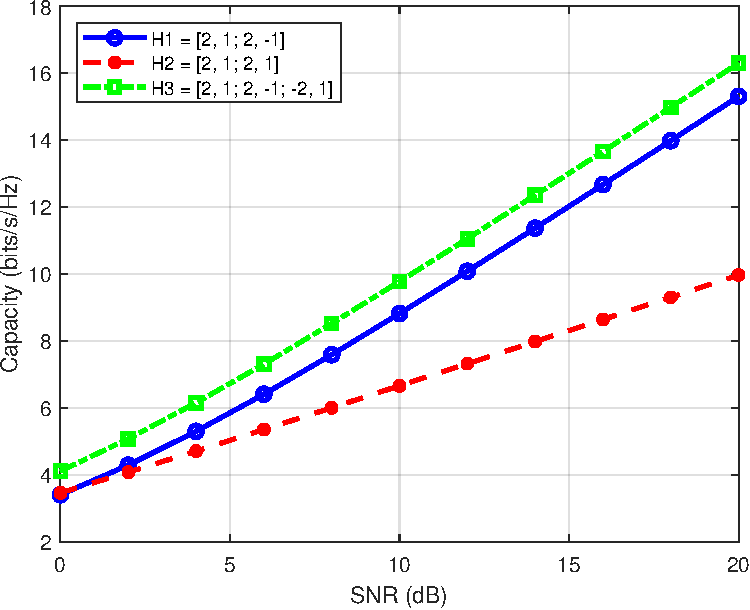
\includegraphics[width=2.5in]{MIMO_Channel_Capacity_vs_SNR}
\caption{Channel Capacity vs. SNR.}
\label{fig:ChannelCapacityvsSNR}
\end{center}
\end{figure}

The simulation results depicted in Fig. \ref{fig:ChannelCapacityvsSNR} demonstrate the channel capacity as a function of SNR for each of the three MIMO channels. The following observations were made:

\begin{enumerate}
    \item The capacity for all channels increases logarithmically with SNR, which is consistent with the Shannon-Hartley theorem. 
    \item For \( \mathbf{H}_1 \) and \( \mathbf{H}_3 \), which have both positive and negative entries, the capacity curves are similar, suggesting that the sign of the off-diagonal elements does not significantly impact the capacity when using the waterfilling algorithm.
    \item Channel \( \mathbf{H}_2 \), with identical off-diagonal elements, exhibits a distinctly lower capacity across the SNR range, illustrating the impact of channel diversity on capacity. A lack of diversity, as indicated by the equal off-diagonal elements, results in a suboptimal configuration for capacity maximization.
    \item The capacity of \( \mathbf{H}_3 \), which has an additional row compared to \( \mathbf{H}_1 \), is not significantly higher. This suggests that simply increasing the number of receive antennas without a corresponding increase in the number of transmit antennas does not necessarily lead to a proportionate increase in capacity, underscoring the importance of channel matrix balance.
\end{enumerate}

The theoretical underpinnings of the waterfilling algorithm suggest that power should be allocated more to the stronger eigenmodes of the channel. This was confirmed through the simulation results, where the algorithm effectively distributed power based on the calculated water level \( \mu \) and the singular values of the channel matrices.

In conclusion, the waterfilling algorithm's efficacy in maximizing the MIMO channel capacity was clearly validated by the simulations. The algorithm adeptly adjusted power allocation in response to the SNR variations and the specific eigenmode structure of each MIMO channel matrix, demonstrating its robustness and adaptability in diverse channel conditions.

\section{Conclusion}

This investigation confirms the efficacy of the waterfilling algorithm in optimizing MIMO channel capacities with CSIT. Simulations show a logarithmic capacity increase with SNR, aligning with the Shannon-Hartley theorem. The algorithm's performance is robust to channel matrix sign variations and highlights the importance of channel diversity. Notably, adding receivers without additional transmitters does not linearly increase capacity, pointing to the need for balanced system design. These findings validate the waterfilling algorithm as an effective tool for enhancing spectral efficiency in wireless communications.

\appendix[MIMO Channel Capacity Waterfilling]

In this appendix, we present the MATLAB code used for calculating the capacity of MIMO channels with the waterfilling algorithm. The code calculates the channel capacities for three different MIMO channel matrices across a range of SNR values.

Below is a snippet of the MATLAB code:

\begin{lstlisting}[language=Matlab]
% MIMO Channel Capacity Calculation using Waterfilling Algorithm

clc;
clear;

% Define the channel matrices
H1 = [2, 1; 2, -1];
H2 = [2, 1; 2, 1];
H3 = [2, 1; 2, -1; -2, 1];

% Define the SNR range from 0 dB to 20 dB with a step of 2 dB
SNR_dB = 0:2:20;

% Initialize arrays to hold capacities for each channel
capacity1 = zeros(1, length(SNR_dB));
capacity2 = zeros(1, length(SNR_dB));
capacity3 = zeros(1, length(SNR_dB));

% Loop over each SNR value
for i = 1:length(SNR_dB)
    % Convert SNR from dB to linear scale
    SNR_linear = 10^(SNR_dB(i) / 10);
    
    % Calculate capacities for each channel matrix
    capacity1(i) = waterfilling_capacity(H1, SNR_linear);
    capacity2(i) = waterfilling_capacity(H2, SNR_linear);
    capacity3(i) = waterfilling_capacity(H3, SNR_linear);
end

% Plotting
figure;
plot(SNR_dB, capacity1, 'b-o', 'LineWidth', 2, 'MarkerSize', 6); hold on;
plot(SNR_dB, capacity2, 'r--*', 'LineWidth', 2, 'MarkerSize', 6);
plot(SNR_dB, capacity3, 'g-.s', 'LineWidth', 2, 'MarkerSize', 6);
xlabel('SNR (dB)');
ylabel('Capacity (bits/s/Hz)');
% title('Channel Capacity vs. SNR');
legend('H1 = [2, 1; 2, -1]', 'H2 = [2, 1; 2, 1]', 'H3 = [2, 1; 2, -1; -2, 1]', 'Location', 'northwest');
grid on;

% Function to calculate capacity using waterfilling for a given channel matrix and SNR
function capacity = waterfilling_capacity(H, SNR_linear)
    % Compute SVD
    [~, Sigma, ~] = svd(H);
    singular_values = diag(Sigma);
    
    % Total transmit power (assumed)
    P_t = 1;  % This value can be adjusted as needed

    % Water-filling algorithm to allocate power
    mu = find_water_level(singular_values, P_t, SNR_linear);

    % Calculating capacity with allocated power
    capacity = 0;
    for i = 1:length(singular_values)
        P_opt = max(mu - 1 / (SNR_linear * singular_values(i)^2), 0);
        capacity = capacity + log2(1 + SNR_linear * singular_values(i)^2 * P_opt);
    end
end

% Function to find the water level for the water-filling algorithm
function mu = find_water_level(singular_values, P_t, SNR_linear)
    mu = 0;
    for v = 0:0.001:10  % This range and step size can be adjusted as needed
        power_sum = 0;
        for i = 1:length(singular_values)
            power_sum = power_sum + max(v - 1 / (SNR_linear * singular_values(i)^2), 0);
        end
        if power_sum <= P_t
            mu = v;
        else
            break;
        end
    end
end

\end{lstlisting}

The code includes functions for calculating the capacity using the waterfilling algorithm and plotting the results. The calculations are based on the SVD of the channel matrices and the SNR values.

\bibliographystyle{IEEEtran}
\bibliography{references}

\end{document}


